\documentclass[10pt,twocolumn,letterpaper]{article}

\usepackage{cvpr}
\usepackage{times}
\usepackage{epsfig}
\usepackage{graphicx}
\usepackage{amsmath}
\usepackage{amssymb}

% Include other packages here, before hyperref.

% If you comment hyperref and then uncomment it, you should delete
% egpaper.aux before re-running latex.  (Or just hit 'q' on the first latex
% run, let it finish, and you should be clear).
\usepackage[breaklinks=true,bookmarks=false]{hyperref}

\cvprfinalcopy % *** Uncomment this line for the final submission

\def\cvprPaperID{****} % *** Enter the CVPR Paper ID here
\def\httilde{\mbox{\tt\raisebox{-.5ex}{\symbol{126}}}}

% Pages are numbered in submission mode, and unnumbered in camera-ready
% \ifcvprfinal\pagestyle{empty}\fi
% \setcounter{page}{4321}
\begin{document}

%%%%%%%%% TITLE
\title{2020 Fall COMP4471 Project Milestone\\Google Landmark Recognition}

\author{LAM Man Hei\\
HKUST\\
{\tt\small mhlamaf@ust.hk}
% For a paper whose authors are all at the same institution,
% omit the following lines up until the closing ``}''.
% Additional authors and addresses can be added with ``\and'',
% just like the second author.
% To save space, use either the email address or home page, not both
\and
LIAO Yi Han\\
HKUST\\
{\tt\small yliaoag@ust.hk}
}

\maketitle
%\thispagestyle{empty}

%%%%%%%%% BODY TEXT
\section{Introduction}
Deep convolution neural network has already gotten remarkable results in image classification tasks. In this project, we are going to investigate landmark recognition with deep convolution neural network, in which we will develop a landmark recognition model for people to better understand and organize their photo collections. We will attempt to use ResNet\cite{he_deep_2015} and EfficientNet\cite{tan_efficientnet_2020} to construct a landmark recognition model. Both model performance will be evaluated, and the best model will be elected as the final landmark recognition model.

%-------------------------------------------------------------------------
\subsection{Problem statement}
The dataset used in this project is retrieved from Google Landmark Recognition 2020\footnote{\url{www.kaggle.com/c/landmark-recognition-2020}}, which is a Kaggle competition. Since the competition is closed and no longer accept submission, the ground truth of the test dataset cannot be retrieved. Thus, only train dataset will be used in this project, and it is split into train, validation and test set. The expected result of the model is a column vector of the probability of each label. The label with the highest probability would be the predicted label of that image. To evaluate the performance of a model, some basic metrics are used, including accuracy, precision, recall, F1-score and confusion matrix.

%------------------------------------------------------------------------
\section{Technical Approach}
To achieve the objective, the following pipeline is proposed. First, exploratory data analysis (EDA) is done with the dataset to have a better understanding of the dataset. After that, some preprocessing work will be done based on the result of EDA. Then, the proposed model, ResNet and EfficientNet, will be trained and evaluated in order to find the best model for landmark recognition.

%-------------------------------------------------------------------------
\subsection{Exploratory Data Analysis}
In exploratory data analysis (EDA), we would inspect the dataset and try to summarize the characteristics of the dataset, such as the property of the images and the balancedness of the dataset. Some graph visualization would be made, such as histogram and box plot, in order to get a better understanding of the dataset.

%-------------------------------------------------------------------------
\subsection{Preprocessing}
In pre-processing, the images is first resize to 224 x 224 in order to fit into the models (ResNet and EfficientNet). Then, apply normalization to the images data. 
To increase the amount of data samples for those landmark classes with extremely limited samples, using data augmentation to enlarge their sample size. It also helps reduce the overfitting problem.

%-------------------------------------------------------------------------
\subsection{Landmark Recognition Model}
In this project, two deep convolution neural networks, ResNet and EfficientNet are tested and evaluated. The models are implemented with PyTorch\cite{paszke_pytorch_2019} along with some common python packages, such as numpy, pandas, and sci-kit learn. Since the dataset is very large, it is time-consuming to train a brand new network due to the limited hardware situation. Therefore, transfer learning technique is applied in order to shorten the training time. The final fully connected layer of the models is replaced with a new fully connected layer with the output size the same as the number of landmarks. Then, the model will be trained for a few epochs.

In the training progress, two loss functions, cross entropy loss and label-distribution-aware margin (LDAM) Loss\cite{cao_learning_2019} are tested. Cross entropy loss is a very common loss function used in classification problem. It can be considered as a baseline loss function. However, the dataset may have data imbalance issue, which cannot be solved by cross entropy loss. Using this loss function with a extreme imbalance dataset may cause low precision/recall in minority class. To get a better representation on minor class, LDAM loss can be use. The loss function is formulated as such:
\begin{align}
    \mathcal{L}_{LDAM}((x, y); f) &= -\log{\frac{e^{z_y - \Delta_y}}{e^{z_y - \Delta_y} + \sum_{j \ne y}e^{z_j}}}\\
    \text{, }\Delta_j &= \frac{C}{n^{1/4}_j} \textbf{ for } j \in [1,k]
\end{align}
where $C$ is a hyperparameter, $n_j$ is the number of sample of $j$-th class, and $z_j$ is the model prediction output of j-th class. By using LDAM loss, it attempts to increase the margin distance of the minority classes from the decision boundary.

In addition, hyperparameters tuning is required in order to obtain an optimized model. Grid search or Bayesian optimization, which is a more efficient technique, is applied to tune model hyperparameters.

%------------------------------------------------------------------------
\subsection{Evaluation}
To evaluate the performance of the deep learning model, accuracy, precision, recall and F1 score would be used.
\begin{align}
    \textbf{Precision} &= \frac{TP}{TP+FP}\\
    \textbf{Recall} &= \frac{TP}{TP+FN}\\
    \textbf{F1} &= 2 \times \frac{\textbf{Precision} \times \textbf{Recall}}{\textbf{Precision} + \textbf{Recall}}
\end{align}
where $TP$, $TN$, $FP$, $FN$ is the number of true positive, true negative, false positive, false negative prediction of the class respectively. Moreover, confusion matrix would be a visual evaluation metric.


%------------------------------------------------------------------------
\section{Preliminary Results}

%------------------------------------------------------------------------
\subsection{Exploratory Data Analysis}
There are $81313$ landmark classes with $1580470$ images in total.

Through EDA, an important feature of the dataset is detected that the dataset is very imbalanced as shown in figure \ref{fig:dist_data}. The largest landmark class sample size is $6272$ while the smallest landmark class sample size is only $2$. Almost $97.5\%$ of the landmark classes are with sample size under 100.  

Besides, the quality of images in the dataset is not very high. There are some quite misleading images even for human beings to recognize. For example, figure \ref{fig:landmark_example} shows how diverse the image in a landmark class can be. 

\begin{figure}[!htb]
    \centering
    % \begin{minipage}[t]{0.23\textwidth}
    %     \includegraphics[width=\textwidth]{img/top12_test_efficientnet.png}
    % \end{minipage}
    \begin{minipage}[t]{0.23\textwidth}
        \includegraphics[width=\textwidth]{img/4440bfd817bfb6c8.jpg}
    \end{minipage}
    \begin{minipage}[t]{0.23\textwidth}
        \includegraphics[width=\textwidth]{img/1115e27655e0f398.jpg}
    \end{minipage}

    % \begin{minipage}[t]{0.23\textwidth}
    %     \includegraphics[width=\textwidth]{img/5cabed3e024e01d8.jpg}
    % \end{minipage}
    % \begin{minipage}[t]{0.23\textwidth}
    %     \includegraphics[width=\textwidth]{img/25f2e0d9c3bb6563.jpg}
    % \end{minipage}

    \caption{Example images of the same class in the dataset. The left image can clearly see the landmark where the right image is just a floor plan.}
    \label{fig:landmark_example}
\end{figure}

\begin{figure}
    \centering
    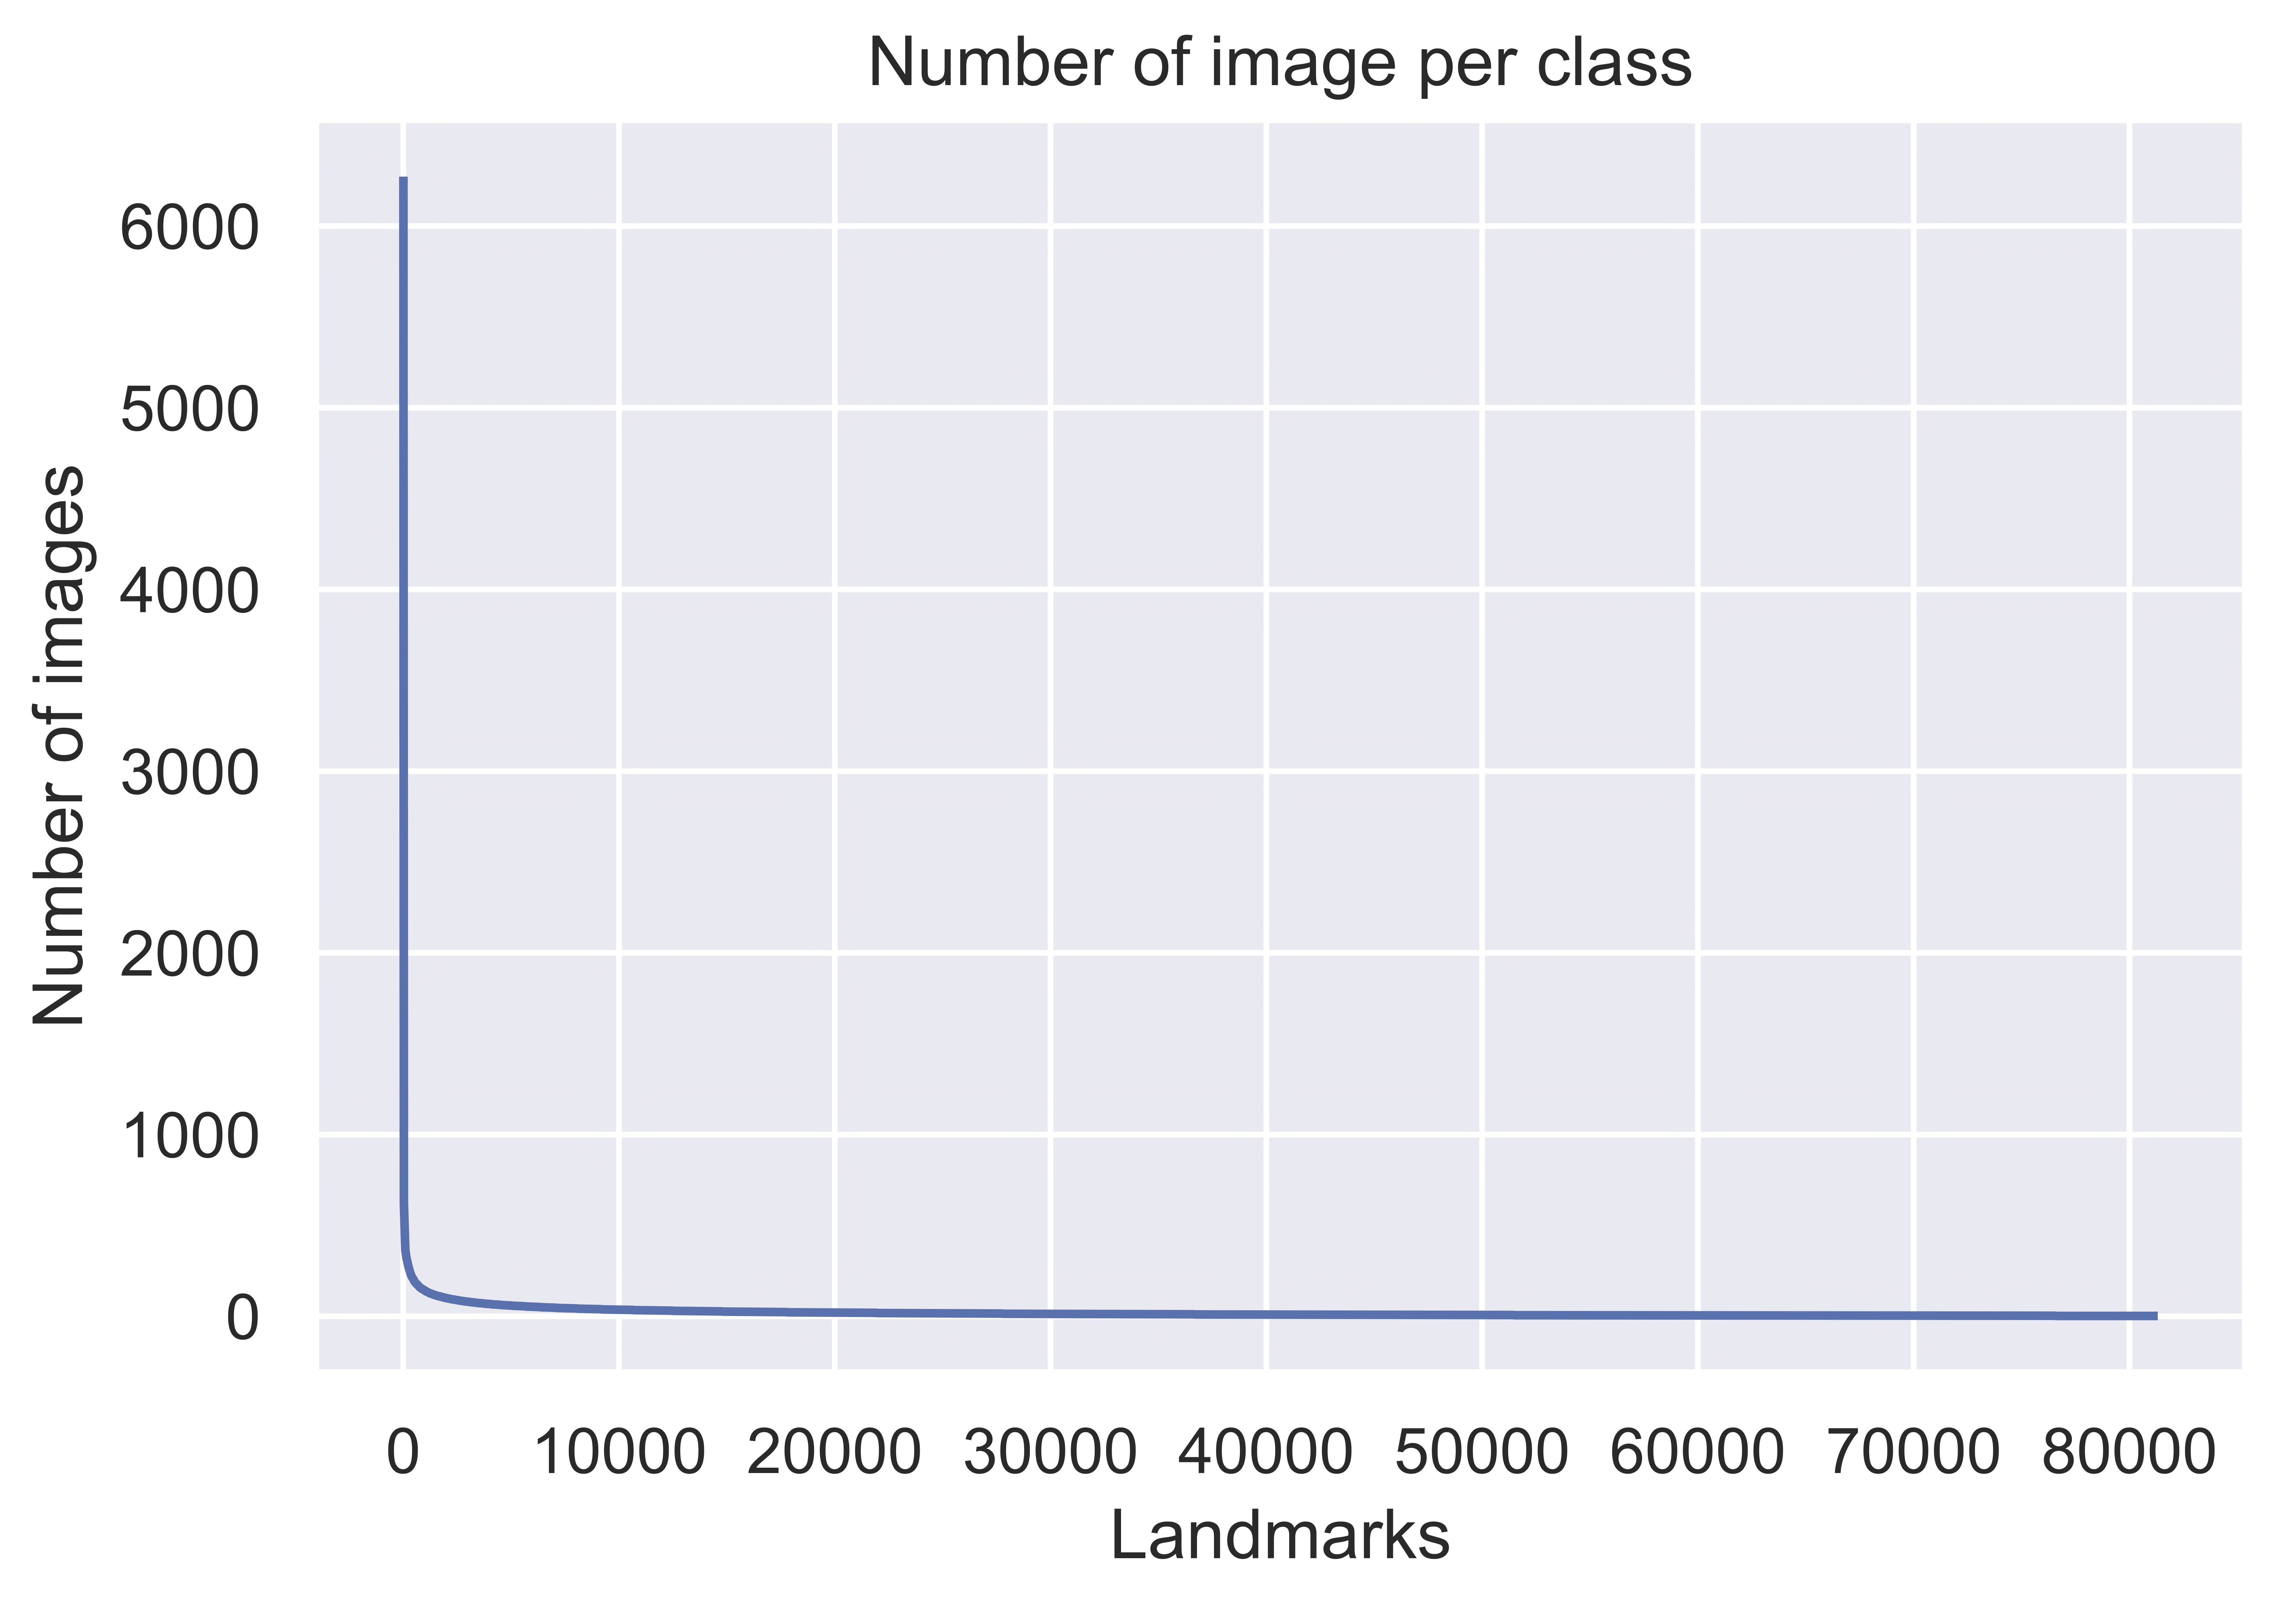
\includegraphics[width=0.5\textwidth]{img/dist.png}
    \caption{Frequency graph of each landmark class. The classes are sorted in descending frequency order.}
    \label{fig:dist_data}
\end{figure}

%------------------------------------------------------------------------
\subsection{Experiment}
Before implementing the model on the whole dataset, top 12 and top 20 landmark classes is first selected to do some experiments. Each sub dataset is split into three parts: training, validation, and testing with the ratio of 0.72, 0.18, 0.1. For both datasets, using ResNet-50 and EfficientNet-B0 as training models and cross-entropy as loss function.

From the performance of these two sub-datasets(table \ref{tab:table1} and table \ref{tab:table2}), we can observe that as more landmark classes are in the dataset, the accuracy will decrease. The main reason is that the minority class has relatively low precision and recall. As shown in the confusion matrix in figure \ref{fig:cm_top20}, the image of landmarks with fewer samples are misclassified as some other landmarks with much more sample. This is a common issue in model training with an imbalance dataset. Therefore, to cope with the dataset with more landmarks and severe imbalance issues, LDAM will be applied to attempt resolving the issue in future works.

\begin{table}[]
    \centering
    \begin{tabular}{c c c}
        \hline Model & Training Accuracy & Testing Accuracy \\ \hline
        ResNet-50 & $98.02\%$ & $96.65\%$ \\
        EfficientNet-B0 & $97.69\%$ & $98.05\%$ \\ \hline
    \end{tabular}
    \vspace{5pt}
    \caption{Model performance of top 12 landmark classes dataset}
    \label{tab:table1}
\end{table}

\begin{table}[]
    \centering
    \begin{tabular}{c c c}
        \hline Model & Training Accuracy & Testing Accuracy \\ \hline
        ResNet-50 & $96.05\%$ & $94\%$ \\
        EfficientNet-B0 & $92.40\%$ & $92.72\%$ \\ \hline
    \end{tabular}
    \vspace{5pt}
    \caption{Model performance of top 20 landmark classes dataset}
    \label{tab:table2}
\end{table}

\begin{figure}
    \centering
    % \begin{minipage}[t]{0.23\textwidth}
    %     \includegraphics[width=\textwidth]{img/top12_test_efficientnet.png}
    % \end{minipage}
    \begin{minipage}[t]{0.4\textwidth}
        \includegraphics[width=\textwidth]{img/top20_test_resnet.png}
    \end{minipage}
    \begin{minipage}[t]{0.4\textwidth}
        \includegraphics[width=\textwidth]{img/top20_test_efficientnet.png}
    \end{minipage}
    \caption{Test set confusion matrix of top-20 landmark classification with ResNet50(top) and EfficientNet-B0(bottom). The larger the landmark id, the fewer the sample that landmark have}
    \label{fig:cm_top20}
\end{figure}

{\small
\bibliographystyle{ieee}
\bibliography{egbib}
}

\end{document}
